\documentclass[11pt]{article}
\usepackage[top=3cm, bottom=3cm, left=3.5cm, right=2.5cm]{geometry}
\linespread{1.5}

\usepackage[danish]{babel}
\usepackage[utf8]{inputenc}
\usepackage{amsmath}
\usepackage{pbox}
\usepackage{graphicx}
\usepackage{wrapfig}

\usepackage{relsize}
\usepackage[electronic]{ifsym}
\usepackage{siunitx}
\usepackage{tikz}
\usepackage{circuitikz}
\usetikzlibrary{decorations.pathmorphing}
\usepackage{tabularx}
\usepackage{float}
\usepackage{caption}
\usepackage{subcaption}
\usepackage{url}
\usepackage{cite}
\usepackage{xcolor}
\usepackage[colorlinks,linkcolor={black},citecolor={blue!50!black},urlcolor={blue!80!black},pdfusetitle=true]{hyperref}
\usepackage{mathptmx}
\usepackage{listings}
\usepackage{mdframed}
\bibliographystyle{plainurl}

\newmdenv[
  topline=false,
  bottomline=false,
	rightline=false,
	linewidth=2pt,
	linecolor=black!30!white,
	fontcolor=black!50!white,
  skipabove=\topsep,
  skipbelow=\topsep
]{mdquote}

\begin{document}

% !TEX root = ../rapport.tex

\begin{titlepage}
	\centering
	\includegraphics[width=1\textwidth]{kapitler/billeder/lowrider.jpg}
	\vspace{1cm}
	{\scshape\Large Semesterprojekt\par}
	\vspace{1.5cm}
	{\huge\bfseries Poleposition\par}
	\vspace{2cm}
	{\Large\itshape Alexander D. Larsen, Frederik N. Larsen, Mikkel L. Olsen, Phillip M. Kyndbøl og Rasmus Haugaard\par}
	\vfill
	Faglig vejleder\par
	\textsc{Jan Petersen}

	\vfill

% Bottom of the page
	{\large 08/02 - 25/05 2016}
\end{titlepage}


\section*{Resumé}
Denne rapport beskriver udviklingen af en selvkørende scalextric bil. Bilen bliver udviklet til at kunne køre selv på en ukendt bane. For at kunne netop dette udvikles et mapning-system til at registrere den ukendte bane. Mapningen bliver lavet vha. et digitalt gyroskop og en omdrejningstæller på motoren. Et motorstyringsprogram udvikles til at bruge mapningen. Der udvikles også en elektromagnet til at skabe downforce på bilen, og en stregdetektor til at registrere startlinjen på banen. Der bliver udviklet et 3D-printet chassis for at få plads til alle justeringerne i bilen. Alle de ting der bliver udviklet til bilen er med henblik på at sætte den hurtigst mulige omgangstid på den ukendte bane. 


\newpage

\tableofcontents

\newpage

% !TEX root = ../rapport.tex
\section{Indledning}

SKRIV INDLEDNING

\newpage


% !TEX root = ../rapport.tex

\section{Problemformulering}

Projektet har til formål at udvikle en mikrocontroller-baseret styring til en racerbil med henblik på at opnå den hurtigste omgangstid på en ukendt bane.
Der vil blive fokuseret på to hovedområder; Den fysiske del samt softwaren. Den fysiske del består af optimering af tophastighed, acceleration, bremselængde og hastighed i sving.
Softwaren skal kunne kortlægge den ukendte bane og styrer bilens motor derefter på baggrund af data fra sensorer.

\begin{itemize}
	\item Design en elektromagnet til at skabe downforce til optimering af svinghastighed og optimering af bremselængde.
	\item Undersøg effekten af fysiske ændringer på bilen f.eks. fastsættelse af affjedring i fht. til optimering af banetider.
	\item Design et optoelektronisk system, der kan registrere en startlinje.
	\item Design en optoelektronisk system, der kan registrere motoromdrejninger.
	\item Udvikle et program, der kortlægger en ukendt bane på baggrund af data fra sensorer.
	\item Udvikle et motorstyringsprogram, der optimerer omgangstiden på baggrund af kortlægningen samt data fra sensorer.
\end{itemize}


% !TEX root = ../rapport.tex

\newpage
\section{Idégenerering}
For at opnå den hurtigste omgangstid skal der være en kombination af den rigtige fysiske opsætning af bilen og en mikrocontroller der fortæller bilen hvordan den skal køre på banen.
Det første der blev undersøgt var de fysiske optimeringer der kunne laves på bilen.

\subsection{Hardware}

\begin{itemize}
\item Forøgelse af acceleration og tophastighed
\item Formindskelse af bremselængde
\item Optimering hastighed igennem sving
\end{itemize}
For at optimere ovenstående er der flere ting der kan overvejes, se figur \ref{fig:mindmap1}.

\begin{figure}[ht]
    \centering
    \includegraphics[width=1\textwidth]{kapitler/billeder/Mindmap1.jpg}
    \caption{Idégenerering til optimering af omgangstid}
    \label{fig:mindmap1}
\end{figure}



\subsection{Software}
Udover de fysiske komponenter i bilen skal bilens omgangstid også optimeres ved hjælp af software.


\begin{figure}[ht]
    \centering
    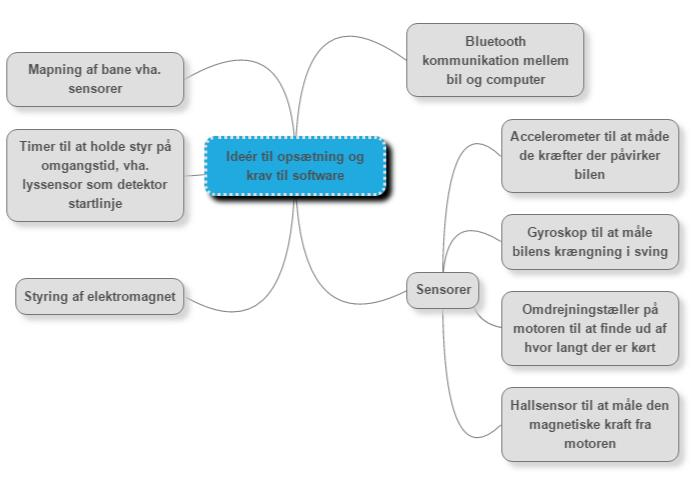
\includegraphics[width=0.8\textwidth]{kapitler/billeder/Mindmap2.jpg}
    \caption{Idégenerering til opsætning af software}
    \label{fig:mindmap2}
\end{figure}


Idéen er, at software skal kunne kortlægge den ukendte bane ved hjælp af sensorer, ved først at kører et par omgange.
Når banen er blevet kortlagt og gemt i bilens hukommelse kan den sætte en hurtig omgangs tid.
Mikrocontrolleren ved herefter, hvor og hvornår der er et sving, hvor der skal bremse og hvor hårdt den kan accelerere de forskellige steder på banen.
Idéen er altså, at bilen skal optimeres til at køre en så hurtig omgangstid som muligt, ved både at optimere det fysiske på bilen, dens hardware og software.


% !TEX root = ../rapport.tex
\newpage
\section{Fysiske modifikationer og hardware}

For at optimere bilens omgangstid, er der fortaget fysiske modifikationer på bilen.
Som beskrevet i opgaveformulering, var der krav til, der skulle bruges enten en elektromagnet eller en hall-sensor.
Ønsket om yderligere downforce i sving og ved bremsning har gjort, elektromagneten er blevet valgt.
Resten af afsnittet tager afsæt i idégenereringen. Se afsnit \ref{idegen}.

% !TEX root = ../rapport.tex
\subsection{Fysiske modifikationer}

For at minimere vægten af bilen er alt unødvendigt plastik blevet fjernet fra bilen. Grunden til dette kan beskrives vha. Newtons 2. lov. Bilen bevæger sig fremad med en kraft F, og bilen har en masse m. 
\begin{equation}
F=m \cdot a
\end{equation}
\begin{equation}
a = \frac{F}{m}
\end{equation}
Accelerationen a, stiger derved jo mindre massen af bilen er. 

Downforce er ekstremt brugbart i sving da det hjælper med at holde bilen på banen ved højere fart. Downforce er mindre brugbart på lige strækninger da bilen let bliver på banen og downforce faktisk vil sænke bilens acceleration og topfart. Derfor indføres der justerbar downforce med elektromagneten. I det 3D-printet chassis er der en indbygget holder til elektromagneten. Elektromagnet er placeret bagerst for at give kontra til den permamagnet der i forvejen sidder i bilen. Permamagneten er placeret foran og tæt på splitten for at trække splitten ned i banen. For uddybning af elektromagneten se sektion \ref{Elektromagnet}.

\subsubsection{3D-printet chassis}

For at kunne hurtigt gennem sving kræver det et lavt tyngdepunkt i bilen, jo lavere tyngdepunktet er jo hurtigere kan bilen klare at køre gennem et sving uden at kæntre. Dette fænomen kan ses på figur \ref{fig:bilsving} nedenfor.
\begin{figure}[ht]
    \centering
    \includegraphics[width=0.8\linewidth]{kapitler/billeder/bilsving.png}
    \caption{Skitse af bilen i et venstresving med to forskellige tyngdepunkter}
    \label{fig:bilsving}
\end{figure}
På bil 1 er tyngdepunktet (den blå prik) lavt og derved har den en kortere arm (den grønne streg) fra tyngdepunktet til omdrejningspunktet (den røde prik). Omdrejningsmomentet(den lilla pil) kan beskrives som:
\begin{equation}
\tau = F \cdot L
\end{equation}
Hvor $\tau$ er omdrejningsmomentet, L er armen (den grønne streg) og F er kraften der påvirker den (den sorte pil). Der antages at der skal det samme omdrejningsmoment ($\tau$) til at bilen kæntre.
\begin{equation}
F = \frac{\tau}{L}
\end{equation}
Derved kan det ses at når armen, L, bliver større skal der mindre kraft F til bilen kæntre. 
Ved at fjerne affjedringen optimeres tyngdepunktet også da karrosseriet er i sin laveste tilstand hele tiden, og ikke kun når fjedrene er trykket sammen.

Det udleveret chassis på racerbilen er meget vakkelvornt, og kan vrides let. For at optimere dette er der blevet 3D-printet et nyt forstærket chassis. Det chassis er stærkere end det gamle og giver lettere plads til at montere sensorer og aktuatore i bilen. Det nye chassis er tegnet i AutoDesk Inventor og derefter 3D-printet med Makerbot. 3D-printet er printet i flere dele og derefter samlet med skruer. En fordel ved at printet er i flere dele er hvis én del går i stykker skal man ikke printe det hele igen. 3D-tegningen ses på figur \ref{fig:3Dtegning} nedenfor.

\begin{figure}[ht]
    \centering
    \includegraphics[width=0.7\textwidth]{kapitler/billeder/3Dtegning.jpg}
    \caption{3D-tegning af bilens chassis}
    \label{fig:3Dtegning}
\end{figure}


Det vil sige at den affjedring der følger med bilen er blevet fjernet og erstattet med det afstivet chassis. Grunden til man har affjedring i virkelige biler er for at beskytte både kører og motor, da man aldrig er sikker på asfaltens tilstand. Da banen racerbilen skal køre på er flad og der er ingen kører der skal beskyttes, vil det optimere bilens hastighed igennem sving uden at den kæntre, at fjerne affjedringen. På figur \ref{fig:racerchassis} nedenfor ses det 3D-printet chassis med motor og hjul på.

\begin{figure}[ht]
    \centering
    \includegraphics[width=0.7\textwidth]{kapitler/billeder/racerchassis.jpg}
    \caption{3D-printet chassis med motor og hjulakser}
    \label{fig:racerchassis}
\end{figure}

Det nye 3D-printet chassis er også udviklet til at ATmega-boardet kan skrues direkte på. Det nye chassis er blevet testet mod det gamle chassis i et 180 graders sving. Med det gamle chassis var den maksimale indgangshastighed bilen kunne køre ind i et sving uden at ryge af 1.9 m/s. Med det nye chassis kan bilen kører samme sving med en indgangshastighed på 2.6 m/s uden at ryge af.

% !TEX root = ../rapport.tex

\subsection{Elektromagnet}
\label{Elektromagnet}

%"Har lavet flere kommentare i  sån så alle i gruppen lige er opmæksomme på det, har gemt et indivuduelt tekst dokument så det kan genlæses, ellers slettes disse bare når i har læst dem "

Elektromagnetens formål er at give bilen ekstra nedadrettet kraft i svingende, således at bilen kan køre hurtigere rundt i svinget, og i sidste ende køre en hurtigere omgangstid. Se afsnit \ref{fysiske-modifik}. Dette kan gøres da racerbanen der køres på har 2 stål skinner i midten af banen.

Da det ikke er fordelagtig at havde ekstra downforce i løbet af længere lige strækninger, grundet den unødig ekstra friktion det vil skabe, skal magneten også kunne slås til og fra. Dette er blevet udført ved at styre elektromagneten med en mosfet der er koblet til mikrocontrolleren. Det bliver ud fra mikrocontrolleren sendt en puls med ca. 30 kHz til mosfett’en og da spolen vil modvirke momentane ændringer, vil den opfatte det som en DC strøm, der varigere efter ønsket duty cykle. Dette gør at man kan undgå at spolen bliver for varm, men også at intensiteten af elektromagneten kan kontrolleres.
%"Har snakket med Jan og der kommer kun kompleksemodstande ved en sinus signal, men vi sender det der hedder transient signal / firkantet signal, og spolen modvirker jo de her momentane ændringer. Slet når læst "

Berigninger på at mosfetten ikke bliver for varm kan ses på bilag \ref{subsec:mosfet}.

\subsubsection{Størrelse}

Dette medføre at elektromagneten først og fremmest er begrænset af bilens dimensioner, da der ønskes at lave den så kraftig som mulig. I det special lavet chasiss er der et frirum på bredden 1.5cm, højden 1.5 cm og længden 1.5 cm. Altså et total volume for hele elektromagneten på 3.375 $cm^3$
%"Ved godt det ikke helt er det, men i stedet for at fylde rapporten ud med meget tid og plads fyldende beregninger på noget så kedligt som volume og for at holde fokus på det vigtige om elektromagneten er dette valgt. slettes når læst"

Elektromagnetens kerne er af stål, og har en total volumen på 0.645 $cm^3$ giver det os resterne 2.73 $cm^3$ til spolen.
%"kernens 2 ben=2*1.5*1.5*0.1 cm + kernen del hvorpå spolen sidder 0.1*1.3*1.5.  slettes når læst "

Dette kan bruges til at estimere hvor mange vindinger N, vi kan havde med en ledning med tværsnitsareal $A_w$, med en spole med gennemsnit radius på r som er 0.45 cm.  $l_{spole}$ er længden af ledningen viklet om spolen.
%"Gennemsnit omkreds da omkredsen stiger linært i takt med der kommer viklinger. 0.3cm for kernen, spole slutter ved 0.6cm det giver gns på 0.45 cm….. *Givet at viklingerne ligger helt tæt.. slettes når læst "

\begin{equation}
Vol_{max} =l_{spole} \cdot A_w = 2\pi \cdot r \cdot N \cdot A_w
\end{equation}
\begin{equation}
N= \frac{Vol_{max}}{2\pi \cdot r \cdot A_w}
\end{equation}

Til elektromagneten i dette projekt blev der brugt en 0.2 mm kobberledning, da spolen let spindes på maskine uden at lakeringen blev skrabet af og kortslutninger fremkom. Dog et skridt der let kunne optimere elektromagnetens ydeevne da en tyndere ledning ville resultere i flere viklinger. Dog skal man være opmærksom på man ikke sender for meget strøm igennem ledningen end den kan holde til.
%"Slettes evt. hvis vi ikke ønsker at skulle snakke om resitivitet til eksamen mm. Har dog ikke nogle gode nok beregninger til at kunne tages med i rapporten."

Teoretisk vil dette medføre en spole om kernen med følgende antal vindinger:

\begin{equation}
N=\frac{2.73*10^{-6} m^3}{0.0045m*\pi*2*((0.0002m)^{2}*\pi)} = 769 vindinger
\end{equation}
I praksis blev der dog kun plads til 600 vindinger.

\subsubsection{Kraft}

Den kraft denne elektromagnet vil kunne trække bilen ned med kan estimeres ved først at kigge på den magnetiske energi $W_m$, der vil blive opladt i en mængde materiale $ \Delta V$ med en konstant permeabilitet $ \mu $. \cite{FysBog}

\begin{equation}
W_m =\frac{B^2}{2 \mu} \Delta V
\end{equation}

Hvis man integrere energi densiteten over volumen af hele det magnetiske kredsløb og antager at B-feltet bliver holdt konstant igennem tværsnits arealet A på elektromagneten, medføre det at:

\begin{equation}
\Phi=B*A
\end{equation}
\begin{equation}
B=\frac{\Phi}{A}
\end{equation}

\begin{equation}
W_m = \frac{1}{2} \int B^2 \frac{dv}{\mu}  = \frac{1}{2} \Phi^2 \int \frac{1}{A^2 \cdot \mu} dV
\end{equation}

Det gælder for et magnetisk kredsløb at den resulterende flux $\Phi$ kan regnes som:

\begin{equation}
\Phi \simeq \frac{NI}{R_m} \simeq  \frac{NI}{\frac{1}{A\mu_0}}
\end{equation}

$N \cdot I$ er ampere vindinger, $R_m$ er kredsløbets totale reluktans, $ \mu $ er kredsløbets permeabilit og l er længden af kredsløbet. Det gælder for kredsløbet at:

\begin{equation}
\Delta V =A \cdot dl
\end{equation}

Det medføre at kredsløbets energi kan skrives som:

\begin{equation}
W_m = (NI)^2/(2(R_m)^2) \int \frac{dl}{A \cdot \mu}
\label{fig:wm}
\end{equation}

Det gælder at den samlede reluktans er summen af alle reluktanserne, i kredsløbet.

\begin{equation}
R_m = \int \frac{dl}{A \cdot \mu}
\label{fig:rm}
\end{equation}

Sammensættes lignin \ref{fig:rm} og \ref{fig:wm} fås:

\begin{equation}
W_m = \frac{(NI)^2}{2R_m}
\label{wmdone}
\end{equation}

Energi balancen i kredsløbet er.
$mekanisk arbejde + magnetisk energi =Elektrisk energi \cdot tid$

\begin{equation}
F dx + dW_m = iv dt
\label{Fdx}
\end{equation}

Givet at strømmen i spolen kan antages som konstant vil den elektrisk energi skrives som.

\begin{equation}
iv=IN \frac{d\Phi}{dt} =(NI)^2  \frac{d\frac{1}{R_m}}{dt}
\label{iv}
\end{equation}


Sammensættes ligning \ref{wmdone}, \ref{iv} og \ref{Fdx} fås det:

\begin{equation}
F dx+\frac{(NI)^2}{2d} \frac{1}{R_m} =(NI)^2  d \frac{1}{R_m}
\end{equation}

Ud fra dette kan det konstateres at halvdelen af den totale elektriske energi bliver omdannet til mekanisk arbejde.

\begin{equation}
F = \frac{dR_m}{dx} (-\frac{1}{2} (\frac{(NI)}{Rm} )^2 )
\end{equation}

Hvor x er elektromagnetens længde fra skinnen ganget med 2, da vi har en hesteformet magnet.

Den samlet reluktans er summen af alle kredsløbets reluktanser, I dette tilfælde vil der være reluktans fra selve elektromagneten $R_k$, fra luftgabet $R_l$ og fra skinnerne i racerbanen $R_s$.

Som det kan ses på figuren fornede.

\begin{figure}[ht]
	\label{fig:Mkreds}
	\centering
	\includegraphics[width=1\textwidth]{kapitler/billeder/EMagnet.jpg}
	\caption{Elektromagnetisk kredsløbs analogi}
	\end{figure}

%Tegnes Lørdag eller søndag beklager ventetiden.

\begin{equation}
\label{rm1}
R_m =R_k + R_s + R_l = \frac{l_{kerne}}{\mu_{r.staal} \cdot \mu_0 \cdot A_{kerne} } + \frac{l_{skinne}}{\mu_{r.staal} \cdot \mu_0 \cdot A_{skinne} }  + \frac{l_{kerne}}{\mu_0 \cdot A_{luftgab} }
\end{equation}

Hvor l står for henholdsvis længden af kernen, skinnen og luftgabet. A for tværsnitsarealet,og $ \mu_{r.staal} $ for den relative permeabilitet til forhold luftens permeabilitet $\mu_0$.  For at forsimple udtrykket kan den totale reluktans sammenlignes med luftgabets reluktans en værdi  der fremover bliver kaldt z.

\begin{equation}
z = \frac{R_m}{R_l} = \frac{R_k}{R_l} +\frac{R_s}{R_l} + 1 = \frac{
\frac{l_{kerne}}{l_{luftgab}} }
	{\mu_{r.staal} \cdot \frac{A_{kerne}}{A_{luftgab}} }
+
\frac{
	\frac{l_{skinne}}{l_{luftgab}} }
{\mu_{r.staal} \cdot \frac{A_{skinne}}{A_{luftgab}} }
+ 1
\end{equation}
%"Motherfucker equation... i know, men den er meget væsentlig og burde ikke skrives kortere"

Ved en lille fluxspredning vil det kunne antages at.

\begin{equation}
A_{kerne} \simeq A_{luftgab}
\end{equation}
\begin{equation}
A_{skinne} \ll A_{luftgab}
\end{equation}

Og idet at der tilføjes elektrisk stål til elektromagnetens kerne og det gælder at:
%"leder stadig efter en god kilde på permabiliteter... en der er bedre end wiki..."

\begin{equation}
\mu_{staal} \ll \mu_{Estaal}
\end{equation}
\begin{equation}
  \frac{\frac{l_{kerne}}{l_{luftgab}}}{
  	{\mu_{r.Estaal} \cdot \frac{A_{kerne}}{A_{luftgab}} }} \ll \frac{
	\frac{l_{skinne}}{l_{luftgab}} }
{\mu_{r.staal} \cdot \frac{A_{skinne}}{A_{luftgab}} }
\end{equation}

Medføre dette at vi vælger kernen reluktans kan negligere, således kan det redfærdigøres at omskrive ligningen til følgende.

\begin{equation}
z =
\frac{
	\frac{l_{skinne}}{l_{luftgab}} }
{\mu_{r.staal} \cdot \frac{A_{skinne}}{A_{luftgab}} }
+ 1
\end{equation}

Hvis skinnens reluktans undersøges nærmere ses følgende.

%" Rs Ganges og divideres med Lluftagab/Aluftab, da det en korrekt matematisk indgreb der ikke ændre værdien af Rs men gør vi kan sammenligne Rs og Rl… slettes når læst. "

\begin{equation}
R_s =  \frac{l_{skinne}}{\mu_{r.staal} \cdot \mu_0 \cdot A_{skinne} }
=
\frac{
	\frac{l_{skinne}}{l_{luftgab}} }{\mu_{r.staal} \cdot \frac{A_{skinne}}{A_{luftgab}} }\cdot \frac{l_{luftgab}}{\mu_0 \cdot A_{luftgab}}=\frac{
	\frac{l_{skinne}}{l_{luftgab}} }
	{\mu_{r.staal}\cdot\frac{A_{skinne}}{A_{luftgab}}}\cdot R_{luftgab}
\end{equation}


Da elektromagneten er sænket så meget som muligt holdes den ca. 0.5 mm over skinnen, og skinnens tværsnit fås til $2mm \cdot 4mm$ kan følgende observeres.

\begin{equation}
R_s =
\frac{\frac{15 mm}{1 mm} }
{ 500 \cdot R_{luftgab} }= 0.06\cdot R_{Luftgab}
	\end{equation}

Dette betyder at for dette kredsløbs funktion kan det med rimelighed antages at:

\begin{equation}
R_m \simeq R_l
	\end{equation}

Dette medføre at ligning \ref{rm1} kan skrives som:

\begin{equation}
\mid F \mid = \frac{(NI)^(2) \cdot \mu_0 \cdot A_luftgab } {2 \dot x^2}
\end{equation}

Det kan derfor ses at for at optimere magneten vil de mest betydende led være amperevindinger om magneten og længden af luftgabet.

For magneten der er anvendt til projektet vil den teoretiske kraft, magneten ville genere ved 1 A, placeret 0.5 mm over banen være: %(OBS x=2*placering over banen… slet når læst)

\begin{equation}
\mid F \mid = \frac{(600 amperevindinger)^2 \cdot \mu_0 \cdot 1.5 \cdot 10^{-5} m^2 } {2 \dot (0.001m)^2}
\end{equation}

I praksis kunne magneten ved 0.5 mm placering over skinnen dog kun trække  1.69 N. Det tyder at alle antagelserne gjort har haft større indflydelse end forventet.

\subsubsection{Forsøg}
Da permabiliteten for stål er relativ lav tilforhold fks. Elektrisk stål, er der blevet forsøg at tilsætte elektrisk stål til elektromagnetens kerne. Efter forsøg hvor magneten blev placeret på skinnen, kunne det konkluderes at tilføje Elektriskstål til magnetens kerne kunne forøge den kraft elektromagneten kunne trække sig mod skinnen med.
Ved forsøget var magneterne placeret på skinnen. Se figur \ref{fig:Magnet}

\begin{figure}[ht]
	\centering
	\includegraphics[width=1\textwidth]{kapitler/billeder/Magnet.png}
	\caption{Gennemsnitsresultat fra forsøg}
	\label{fig:Magnet}
\end{figure}


\subsubsection{Delkonklusion}
Da amperevindinger efter vores formel skulle havde stor betydning for elektromagnetens kraft er kernen på elektromagneten lavet af et tyndt stykke stål der kun er 1 mm tykt for at få plads til så mange vindinger som muligt. Da ståls permeabilitet ikke er lige så god som for eksempel jern eller elektriskståls, blev der ekspermiteret med at tilføje elektrisk stål til kernen, hvilket gav gode resultater. Den endelige magnet placeret i bilen endte med at trække 1.69 N.

Udover amperevindinger havde magnetens placering fra skinnerne på racerbanen også stor betydning. Dette blev der taget højde for ved at placere elektromagneten så tæt på skinnen som muligt. Ud fra tests, blev en placering på 0.5 mm over banen den bedste. Her blev der ikke skabt for meget bremsende friktion og med lidt tape på undersiden af magneten kortsluttede banen ikke ved ujævnheder i banen.

% !TEX root = ../rapport.tex

\subsection{Bremsefunktion (H-bro)}

Ligesom acceleration, er bremselængden en vigtig faktor for at opnå en god omgangstid.
Når bilen nærmer sig et sving, handler det om at komme så tæt på svinget som muligt, før at bilen
skal begynde at bremse. Dette kræver en effektiv bremse, så bremselængden minimeres og omgangstiden effektiviseres.
For at bremse bilen så effektivt som muligt, benyttes princippet bag en H-bro. Dette princip er illusteret
på figur \ref{fig:hbro}, nedenfor.

\begin{figure}[ht]
    \centering
    \includegraphics[width=1\textwidth]{kapitler/billeder/hbro.png}
    \caption{Viser princippet bag en H-bro, og hvordan den benyttes i dette projekt.}
    \label{fig:hbro}
\end{figure}

Som illusteret på figur \ref{fig:hbro}, kan man bruge en H-bro til at vende strømmen igennem motoren.
Ved at vende strømmen igennem motoren i få millisekunder, vil motoren prøve at bakke,
og bilen vil bremse meget effektivt. Figuren viser det to scenarier, hvor strømmen til højre er vendt
og strømmen til venstre ikke er vendt.

H-broen konstrueres med et dobbelt relæ, som vender de to kontakter når spolen inducere en strøm.
Spolen kræver en høj aktiveres spændning for at trække den nødvendige strøm
og kredsløbet bygges derfor op med en transistor.
Transistoren kan aktiveres med en meget lille strøm og spændning, og kan derfor aktiveres
af ATmega'ens I/O pins.

Bilens motor kan derved bremses, ved at sætte en I/O pin høj, og derved vende strømmen igennem motoren.

(Eventuelt beskrivelse af komponenterne vi har brugt + at nævne det kan skade gearingen.)

% !TEX root = ../rapport.tex
\newpage
\subsection{Boost converter}
En boost converter er et analogt DC-DC kredsløb som har en højere udgangsspænding end indgangsspænding.
Idéen med en boost converter er at øge effekten hen over motoren og derved få højere acceleration og tophastighed. Ved 15V trækker motoren kun 0,5A og derved bruger den kun 7.5 Watt. Da vi har en strømforsyning der kan levere 30 Watt kan vi udnytte det meget mere ved at øge spændingen. Dette vil dog gøre vi ikke helt kan trække 30 Watt da man aldrig kan lave en 100 procent effektiv boost converter.  Ideén er at have en udgangsspænding på 30V, og hvis boost converteren kun er 85 procent effektiv giver det en strøm, I på:
\begin{equation}
15V \cdot 2A = 30 W
\end{equation}
\begin{equation}
30 W \cdot 0,85 = 25,5 W
\end{equation}
\begin{equation}
I = \frac{25,5 W}{30 V} = 0,85A
\end{equation}
Hvilket burde være mere end rigeligt til at drive motoren langt hurtigere end med 15V og 0,5A

\begin{figure}[ht]
    \centering
    \includegraphics[width=0.8\linewidth]{kapitler/billeder/BoostConverter.png}
    \caption{Skematisk tegning af en boost-converter}
    \label{fig:boostconvert}
\end{figure}

På figur \ref{fig:boostconvert} ses et forsimplet kredsløb af en boost converter. Idéen er at når switchen S, sluttes bliver der en magnetisk kraft opladet i spolen L. Når switchen bliver brudt vil kraften fra spolen oplade kondensatoren, men da strømmen i en spole ikke kan ændres momentant vil der også løbe strøm fra spændingskilden igennem spolen og derved vil der opnås en højere spænding over kondensatoren C.

Da dette kredsløb gerne skulle være selvkørende bruges der ikke en switch, men en MOSFET som skal aktiveres af et højfrekvent signal. Det er vigtig at frekvensen er så høj at spolen ikke når at gå i mætning, som vil sige at det ikke når det punkt hvor virker som en kortslutning, da kredsløbet så ville være en direkte kortslutning fra vores spændingskilde til ground.

Det er vigtigt at udvælge de rigtige komponenter til dette kredsløb da det er et højfrekvent kredsløb hvor der løber store strømme. En schottky-diode benyttes da den kan switche ved langt højere frekvenser end en almindelig diode og har et lavere spændingstab henover den og dermed får vi større effektivitet. Kondensator skal have så stor kapitans som mulig(selvfølgelig inden for rimelighedens grænser) og kunne tåle høje spændinger hen over den. MOSFET'en som bliver brugt som switch skal kunne switche hurtigt og kunne klare at der løber stor strøm igennem den uden at blive alt for varm.

En af de problemer ved at bygge en boost converter som fast skal kunne levere 30V er an på motorens hastighed ændre motorens indre modstand sig, og derved ændrer spændingen sig også. Det er derfor nødvendigt at have en form for feedback der fortæller frekvensgeneratoren om den skal øge eller sinke frekvensen for at outputtet bliver som forventet. Der findes IC-kredse der gør dette automatisk, men da gruppen ikke kan stå indenfor hvordan de IC-kredse virker er der blevet valgt ikke at bruge dem i  bilen, og derved ville det blive for stor en udfordring at bygge boost converteren i forhold til den tid der var til projektet.  


% !TEX root = ../rapport.tex

\subsection{Sensorer}


\subsubsection{Stregsensor}
Formålet med stregsensoren er at detektere målstregen. Dette gøres optisk, da selve banen er sort, og målstregen er hvid. Da hvid reflektere lys meget bedre end sort får vi et signal der er let at komparere.

Stregsensoren er bygget op som vist på ref diagram. Den fungere ved at dioden lyser ned på banen, det lys der bliver reflekteret modtager phototransistoren. Ved målstregen har den et output på 4.8 V og på resten af banen 2.5 V. Til at komparere er der blevet brugt en schmitt trigger, således at der kommer en hysterese. Dette er valgt for at undgå at registrere målstregen flere gange i det vi passere den. Reference spændingen ved det inverterende ben på schmitt-triggeren er sat til 3,3 V og hysteresen som vist på figur nedenunder.
\\
Indsæt hysterese kurv*
\\
Stregsensoren sender et signal, ved målstregen på 4.9 V som  mikrocontrolleren modtager som et logisk højt signal. Ved placering over den sorte del af banen sender stregsensoren et signal på 0.03V som mikrocontrolleren opfatter som et logisk lavt signal. 

Ved placering over metalskinnerne på banen sender sensoren også et logisk højt signal, for at undgå at modtage den støj, er sensoren placeret bag venstre forhjul, det gør også at mikrocontrolleren modtager signalet om målstregen hurtigere end hvis den var placeret bagerst på bilen. 

Da det er fordelagtig at havde så lidt vægt i bilen, og for at skabe så meget plads som muligt til blandt andet elektromagneten, er det blevet lavet med SMD-komponenter. 


\subsubsection{Motor-Omdrejningstæller}

For at måle distancer, så bilen ved hvor langt der er imellem sving på banen, er der blevet lavet en omdrejningstæller. Til dette kan samme kredsløb som stregsensoren anvendes, idet der er blevet fremstillet en rotations enkoder, der er fastspændt på motorens akse. Dog er modstanden under transistoren ændret få at gøre sensoren mindre følsom.   


\begin{figure}[ht]
    \centering
    \includegraphics[width=0.4\linewidth]{kapitler/billeder/dekoder.png}
    \caption{3D-tegning af optisk dekoder}
    \label{fig:dekoder}
\end{figure}


Det vil sige at omdrejningstælleren vil sende et logisk højt signal til mikrocontrolleren når den er ved et af hullerne i  rotationsenkoderen, og et logisk lavt signal resten af tiden. En puls fra Omdrejningstælleren vil svare til 1/6 af en motoromdrejning.
Da denne sensor kommer til at blive brugt i flere frekvensområder alt efter motorens hastighed, er det vigtigt at komparatoren ikke er ?begrænset af dens slewrate eller bandwith. ? 


??
Den komperator der er blevet brugt i kredsløbet er en LM311 har ved normal opsætning en respons tid på 165 ns fra høj til lav og 115 ns fra lav til høj.

\begin{equation}
\frac{1 V}{280 ns} = 3.571.429 \frac{v}{s}
\end{equation}

Hvor signalet ved motor omdrejninger ved 2 kHz vil give 12 pulser, det giver et signal der går fra 5 til 0 og 0 til 5 volt med 12 kHz.
\begin{equation}
\frac{10 V}{(12 \cdot 10^-3)s} = 833 v/s
\end{equation}


?? for vagt?? 



Kilde til datasheet: http://www.ti.com/lit/ds/symlink/lm311.pdf


?Hastighed?

inkoder som hver puls fra inkoderen svare til en 1/6 af en motor omdrejning. 

\subsection{Delkonklusion}
De fysiske ændringer der er lavet på bilen optimere næsten alle krav der var stillet inden udviklingen af de enkelte ting blev påbegyndt.
Minimering af vægt blev gjort ved at fjerne alt unødvendigt plastik fra bilen og printe et nyt lettere chassis.
Justerbar downforce blev indført vha. en elektromagnet. Tyngdepunktet blev sænket med det nye chassis der samtid afstivet bilen.
Bremselængde blev kraftig minimeret vha. h-broen dog skal man være opmærksom på at tandhjulene ikke kan holde til at man give motoren for meget fart i modsat retning af køreretningen.
2Accelerationen og tophastigheden blev ikke optimeret da en boost converter blev vurderet til at være for tidskrævende i forhold til projektet.

% !TEX root = ../rapport.tex

\section{Software}
Nu er bilen optimeret mest muligt rent hardwaremæssigt. For at kunne kører den hurtigst muligt omgangstid skal der også udvikles noget sofware. Softwaren skal henholdsvis bruges til at:
\begin{itemize}
\item Kommunikere med bluetooth.
\item Kommunikere med sensorer.
\item Aflæsning af optisk dekoder og stregdetektor.
\item Lave et map af den ukendte bane.
\item Styre motoren i forhold til det gemte map.
\end{itemize}
Alt software til bilen er udviklet i assembly.


% !TEX root = ../rapport.tex
\section{Bootloader}
Programmerstikket til mikroprocessoren er ikke nem at tilgå, når bilen er fuldt monteret. For at kunne iterere hurtigt og undgå at skulle skille bilen ad og samle bilen hele tiden, blev der udviklet en bootloader.

\subsection{Bluetooth}
For at sikre, der kan skabes kontakt med bootloaderen, styrer bootloaderen bluetoothkommunikationen.
\subsubsection{Baudrate}
En række stresstests blev udført for at finde den hurtigste, stabile baudrate mellem mikrocontrollerens og bluetoothmodulet. Dataflowet er primært fra mikrocontrollerens til pc. Stresstestene er opbygget derefter.
En enkelt byte med værdien, x, sendes til mikrocontrollerens, hvorefter mikrocontrollerens sender x kb tilbage.
Se ``avr/src/bt/tests/replykb.asm''.
Forskellige baudrates blev stresstestet ved 250 kB. Den højeste af disse, der ikke havde datatab, var 38 kbps. Disse tests blev udført uden parity bit, med én stop bit og med 8 databits. Det er også denne opsætning der antages fremadrettet. Se eventuelt ``avr/src/bt/bt\_setup.asm''. Det vil sige 9 bits i alt per overført byte. Det giver en teoretisk overførselshastighed på $38 kbps / 9 bpB \simeq 4.2 kB/s$ Der kunne have været eksperimenteret med parity bits og flere stopbits ved højere baudrates, men der var ikke umiddelbart behov for hurtigere overførselshastigheder.
\subsubsection{Output Buffer}
Med en clockfrekvens på 16 MHz går der $16*10^6 / 4.2*10^3 \simeq 3810$ cycles mellem, der kan sende bytes. Hvis man ønsker at sende $x$ bytes synkront, skal programmet i alt vente $(x-1)*3810$ cycles. For at udnytte disse cycles i stedet for at vente, implementeres en buffer i sram.
Se ``avr/src/bt/bt\_tr.asm''.
Bufferen består af en byte liste med en fast længde allokeret i sram samt to pointers, der også er allokeret i sram. Listen indeholder de bytes, der ønskes sendt, samt den frie plads i bufferen. Bytes i det frie område kan være bytes, der allerede er sendt, eller bytes, der endnu ikke er blevet skrevet over siden mikrocontrollerens sidste reset. En store pointer peger på den byte i listen, der blev tilføjet sidst. En send pointer peger på den byte i listen, der blev sendt sidst.
I initialiseringen af bufferen sættes de to pointere til at pege på den samme byte i listen.
Når der ønskes en byte sendt, inkrementeres store pointeren, og byten skrives til den adresse i listen store pointeren repræsenterer. Interrupt enableren for når UART data registeret er tomt sættes højt, så bufferen bliver informeret, når der kan sendes en byte.
Når der kan sendes en byte, og der er bytes i bufferen, der endnu ikke er sendt (store pointeren og send pointeren har ikke samme værdi), inkrementeres send pointeren, og den byte, send pointeren peger på sendes.

Hvis en af pointerne, efter at blive inkrementeret, peger på byten lige efter listens sidste byte, sættes pointeren til den første byte i listen.
Hvis store pointeren, efter at blive inkrementeret og eventuelt rykket til den første byte i listen, peger på samme adresse som send pointeren, er der overflow i bufferen. Det håndteres på nuværende tidspunkt ikke.
TODO: Der skal et billede ind her

\subsection{Protokol}
Bootloaderen styrer bluetoothkommunikationen og indeholder en overordnet kommunikationsprotokol.
Den første byte, initial byte, bootloaderen modtager, afgør, hvordan bootloaderen skal håndtere de næstkommende bytes.
85: Set. 85 gemmes som den første byte i inputbufferen. De to næstkommende bytes gemmes også, før der hoppes til kommando interruptet. Herefter forventer bootloaderen en ny initial byte.
87: Ping. Bootloaderen sender 87 tilbage med det samme. Herefter forventer bootloaderen en ny initial byte.

For at undgå at skulle opdatere bootloaderen, hvis der blev implementeret andre kommandoer i applikationsprotokollen, blev der implementeret en variabel kommando med initial byte: 86.
Den næstkommende byte beskriver længden, n, af kommandoen. De derefter næstkommende, n, bytes gemmes i inputbufferen, før der hoppes til kommando interruptet.
Bemærk:
[85, X, X] og [86, 3, 85, X, X] er ekvivalente.
[87] er ping kommandoen til bootloaderen. [86, 1, 87] er en kommando [87] til applikationen.

Længden er kun variabel for bootloaderen. Der gives ingen information til applikationen om længden af kommandoen.

Når der er en hel kommando (liste af bytes) klar til applikationen, hoppes til 0x2A, en udvidelse af interrupt vektor tabellen.

% !TEX root = ../rapport.tex
\newpage
\subsection{I2C kommunikation}
Til at kommunikere med de digitale komponenter, herunder vores udleveret accelerometer og gyroskop, anvendes den kommunikationsprotokol kaldet I2C eller TWI (”two-wire interface”). Navnet ”two-wire interface” kommer af, at hele kommunikationen foregår over kun 2 ledninger, men hvor der samtidig er mulighed for at kommunikere med mange komponenter.

\begin{figure}[ht]
    \centering
    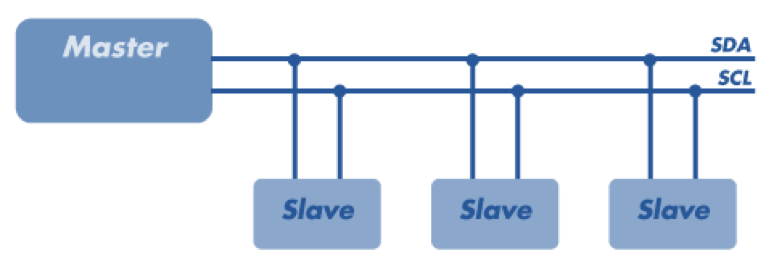
\includegraphics[width=0.8\textwidth]{kapitler/billeder/i2c-princip.png}
    \caption{Viser en skitse af hvordan opsætningen kan laves mellem
én ”master” og flere ”slaver”, kun ved brug af to forbindelser.}
    \label{fig:i2cprincip}
\end{figure}

De to forbindelser der bruges til vores TWI kommunikation hedder SCL (”Serial Clock Line”) og SDA (”Serial Data Line”). SCL er en clock der sættes af master, for at både master og slaven snakker og lytter ved en fælles frekvens. SDA er den forbindelse, hvor alt data bliver overført både fra slaven til master, men også fra master til slaven. Denne form for kommunikation kaldes for halv-duplex, og fungere ligesom en walkie talkie, hvor der kun er én der snakker af gangen, imens den anden lytter.

\subsubsection{Kommunikationsprotokol}

Kommunikationen mellem master og slave, foregår ud fra en bestemt protokol, som er opgivet ved den enkelte slaves datablad. Denne protokol er den samme for accelerometeret og gyroskopet, og er illustreret på figur \ref{fig:i2conebyte}. 

\begin{figure}[ht]
    \centering
    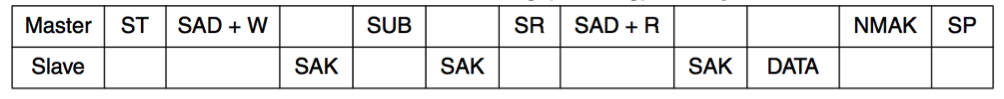
\includegraphics[width=1\textwidth]{kapitler/billeder/i2c-onebyte.png}
    \caption{Kommunikationsprotokol for gyroskopet via I2C}
    \label{fig:i2conebyte}
\end{figure}

Figur \ref{fig:i2conebyte} viser skridt for skridt, hvordan kommunikationsprotokollen er opbygget, hvis man vil læse data én gang fra én af vores to digital komponenter.

Protokollen indeholder følgende instruktioner for at modtage én data byte:

\begin{enumerate}
\item ST (”Start Bit”): Master sender et start bit til alle slaverne, for at starte kommunikationen.
\item SAD+W (”Slave Adress + Write”): Master sender en slave adresse på 7 bits, og det sidste bit beskriver om der skal læses eller skrives, i dette tilfælde skal der skrives. Adressen er specifik for hver komponent og fortæller hvilken slave, som resten af kommunikationen kommer til at foregå med. Det sidste bit indikere, at masteren vil skrive noget til slaven.
\item SAK (”Slave Acknowledge”): Slaven med den valgte adresse sender er ACK bit tilbage, som fortæller at den har hørt hvad masteren sagde, og gør klar til at læse næste instruktions.
\item SUB (”Sub adress”): Master sender herefter en underadresse. Denne underadresse er en 7 bit adresse, som fortæller hvilken register inde i den valgte komponent, der gerne vil adresseres.
\item SAK (”Slave Acknowledge”): Slaven sender endnu et SAK bit, og gør klar til næste instruktion.
\item SR (”Repeated Start”): Master sender herefter et gentagende start bit. Der skal altid sendes en start/repeated start instruktion, hver gang der skiftes mellem at læse eller skrive. Ved repeated start vedholdes forbindelsen til slaven, og slaven ved derfor allerede hvilken underadresse, der herefter skal læses fra.
\item SAD+R (”Slave Adresse + Read”): Master sender herefter igen slave adressen, samt én read bit, for at ændre at vi nu gerne vil læse på slaven, modsat at vores tidligere write, som skrev til slaven.
\item SAK (”Slave Acknowledge”):  Slaven sender en ACK bit.
\item DATA (”Data Byte”): Slaven sender efterfølgende en data byte til master.
\item NMAK (”Master Not Acknowledge”): Herefter sendes én NMAK fra master til slaven, for at indikere at der ikke skal læses mere data.
\item SP (”Stop Bit”): Til sidst sender master et stop bit, for at afslutte kommunikationen.
\end{enumerate}

% !TEX root = ../rapport.tex
\newpage
\section{Lap timer}
Formålet med Lap timeren er at have et stykke kode som måler og returnere omgangstiden, for hver omgang bilen køre. Lap timeren er baseret på "timer1" og er derfor den største timer. Lap timeren bliver udover omgangstid, også brugt af andre kode moduler, til at tage tid.
\subsection{Opsætning af Lap timer}
\subsection{Kode}
\subsection{Macro's}

* Valg af prescaler (udregninger)\\
	-præcision
	-maks/min omgangs tider 
	
* 24-bit register\\
% !TEX root = ../rapport.tex
\newpage

\section{Motor omdrejninger (kode)}

% !TEX root = ../rapport.tex
\newpage
\section{Kortlægning af bane}
Den bedste omgangstid afhænger af mange elektriske komponenter, som bindes sammen af software.
Denne software skal ud fra disse analoge og digital komponenter kunne analysere banen, og ud fra dette
kortlægge banen. Byggestenen til opbygning af denne kortlægning, kan ses på figur \ref{fig:mapflow}.

\begin{wrapfigure}{r}{0.35\textwidth}
  \vspace{-10pt}
  \begin{center}
      \includegraphics[width=0.25\textwidth]{kapitler/billeder/mapflow.png}
    \end{center}
    \vspace{-10pt}
    \caption{Viser grundstenene af koden til kortlægning af banen.}
    \label{fig:mapflow}
\end{wrapfigure}

Som der ses på figur \ref{fig:mapflow}, er pincippet bygget meget simpelt op, og kan beskrives ved følgende punkter:

\begin{itemize}
\item Venter på interrupt fra hvid-streg sensor (Tiltøj til flowchart)
\item Når den hvide streg er registeret, gemmen den omdrejningstælleren.
\item Herefter køres et loop, som bruger gyroskopet til at tjekke om der drejes.
\item Hvis vi drejer, gemmes omdrejningstæller og længden af det lige stykke regnes.
\item Status for et lige stykke, samt længden af stykket gemmes i SRAM.
\item Nyt loop tjekker om svinget er slut. Hvis sving er slut, gemmes omdrejnignstæller.
\item Status for sving, samt længde af sving gemmes i SRAM, og koden starter forfra.
\item Ved næste hvid-streg interrupt stoppes kortlægningen.
\end{itemize}

Når koden er færdig, vil alle sving og lige stykker være defineret i SRAM og koden vil blive behandlet
af et seperat program. 

% !TEX root = ../rapport.tex
\newpage

\subsection{kortlæsning}

Kodemodulet "Kortlæsnings modulet" benytter et map over banen, til at køre efter. Kortlægning kan der læses mere om i afsnit \textbf{kortlægning}.\\

\begin{figure}[ht]
\centering
\includegraphics[width=0.4\textwidth]{kapitler/billeder/mread/mread_ov.png}
\caption{Overordnet flowchart over map read koden}
\label{fig:mread}
\end{figure}

Inden bilen kan køre efter kortet, er det vigtigt at bilen kender sin position på banen. Kodemodulet starter derfor med at finde målstregen, ved brug af streg sensoren. Dernæst indlæses det kommende bane segment. Hvert segment har et status register, som fortæller om det er et sving eller lige stykke. Ud over status registrer, er der også to 8-bit registre som indeholder længden af det pågældende segment. Programmet bruger informationen til at vælge imellem 2 rutiner, rutinen for sving eller rutinen for lige strækninger. Når en af de følgende rutiner er blevet udført og bilen passeret bane segmentet, loades på ny et nyt banesegment.\\
\\
Når rutinen for sving kaldes, tændes elektromagneten for at forbedre grebet. Bilens hastighed bliver sat til den maksimale hastighed for sving.\\
\\
Når rutinen for lige segment kalde, slukkes elektromagneten og hastighed for bilen siddes til max. Ud over det, tjekkes der om næste segment er lige eller et sving. Hvis næste segment er lige, bibeholdes den maksimale hastighed. Hvis næste segment derimod er et sving, beregnes hvornår nedbremsningen skal finde sted, for at nå ned på den maksimale hastighed for sving. Beregningerne for hvornår der skal bremses, sker ved ved at den ønskede bremselængden trækkes fra segmentets længde. Bremselængden er en konstant distance som kan ændres i programmet. Til nedbremsningen benyttes elektromagneten for at skabe mere friktion, samt H-broen til at vende strømmen på motoren.\\



\subsection{Delkonklusion}
Skriv en del konklusion her..

% !TEX root = ../rapport.tex
\section{Diskussion og vurdering}
Produktets kvalitet er vurderet på flere forskellige punkter både de fysiske ændringer og det softwaremæssige. De fysiske ændringer giver en tydelig forbedring af produktet da optimering af tyngdepunkt, placering af magneter og afstivelse af chassis giver en målbar forskel på hastighed gennem sving. Med de nye ændringer kan bilen køre 0.7 m/s hurtigere gennem sving uden af kæntre. De nye ændringer giver også plads til elektromagneten som er yderst optimalt, da den også yder downforce gennem sving. Dermed kan der vurderes at de fysiske ændringer er meget positive og yderst optimale for bilen. 
% !TEX root = ../rapport.tex


\section{Konklusion}


Mikkel skriv noget om elektromagnet her


Det optoelektriske system der blev udviklet til at detektere startlinjen virker optimalt og giver et klart signal gennem schmitt-triggeren. Det samme med motor omdrejningstælleren der også virker optimalt og giver en klar høj-lav puls når motoren kører, og derved en klar indikation om hvor langt bilen har kørt.
Kortlægning af banen er blevet udviklet, for at kunne beregne den bedst mulige omgangstid for bilen.
Denne kortlægning bliver gemt som segmenter i SRAM, for efterfølgende at kunne bliver behandlet.
Ved brug af bane segmenterne og sensorerne styre kortlæsnings modulet: elektromagneten, H-broen og hastigheden. Koden virker som forventet, med maksimal acceleration på lige stykker og samtidig nedbremsning op til sving.
De fysiske ændringer der er blevet fortaget har stor effekt på bilen. Specielt det nedsatte tyngdepunkt, det afstivet chassis og placering af magneter gør at bilen kan tage sving meget hurtigere uden at kæntre.

Samlet giver alle ændringerne at bilen kan kører på ukendt bane, og lave et optimalt forsøg på en hurtig omgangstid.

% !TEX root = ../rapport.tex
\section{Perspektivering}
Med længere tid og flere ressourcer kunne projektet have udviklet sig på flere måder. Som nævnt tidligere kunne en boost converter blive udviklet til at øge spændingen over motoren for at give hurtigere acceleration og højere topfart. Til elektromagnet kunne der have blevet skaffet en jernstang til kerne af magneten, da jern har meget højere permabilitet end stål ville det øge effekten af elektromagneten. 

Permamagneten er ekstremt effektiv i sving og skaber et ekstremt downforce, men på langsider skaber den samme downforce og derfor øger modstanden som bilen skal trække. Ved at have en servomotor der kunne justere permamagnetens afstand fra banen an på om bilen kører ligeud eller drejer. 

\end{document}
